\section{Data Mining Methods}\label{sec:methods}
The encoded table from Section~\ref{sec:preprocessing} is treated as a short sequence of fields, so the model can learn interactions between location, dwelling attributes and time.  The implementation follows the masked-token and self-attention ideas of BERT and the Transformer architecture~\cite{devlin2019bert,vaswani2017attention}; its field-wise input construction is also related to FT-Transformer for tabular data~\cite{gorishniy2021revisiting}.  Figure~\ref{fig:pretrain_finetune} gives an overview: the same BERT backbone is first pretrained to reconstruct masked field tokens and is then fine-tuned with a regression head on \texttt{[CLS]} to predict monthly rent.
% Source: ../../src/bert_rent/model.py; ../../src/bert_rent/data.py; ../../configs/bert.json.

\begin{figure*}[t]
\centering
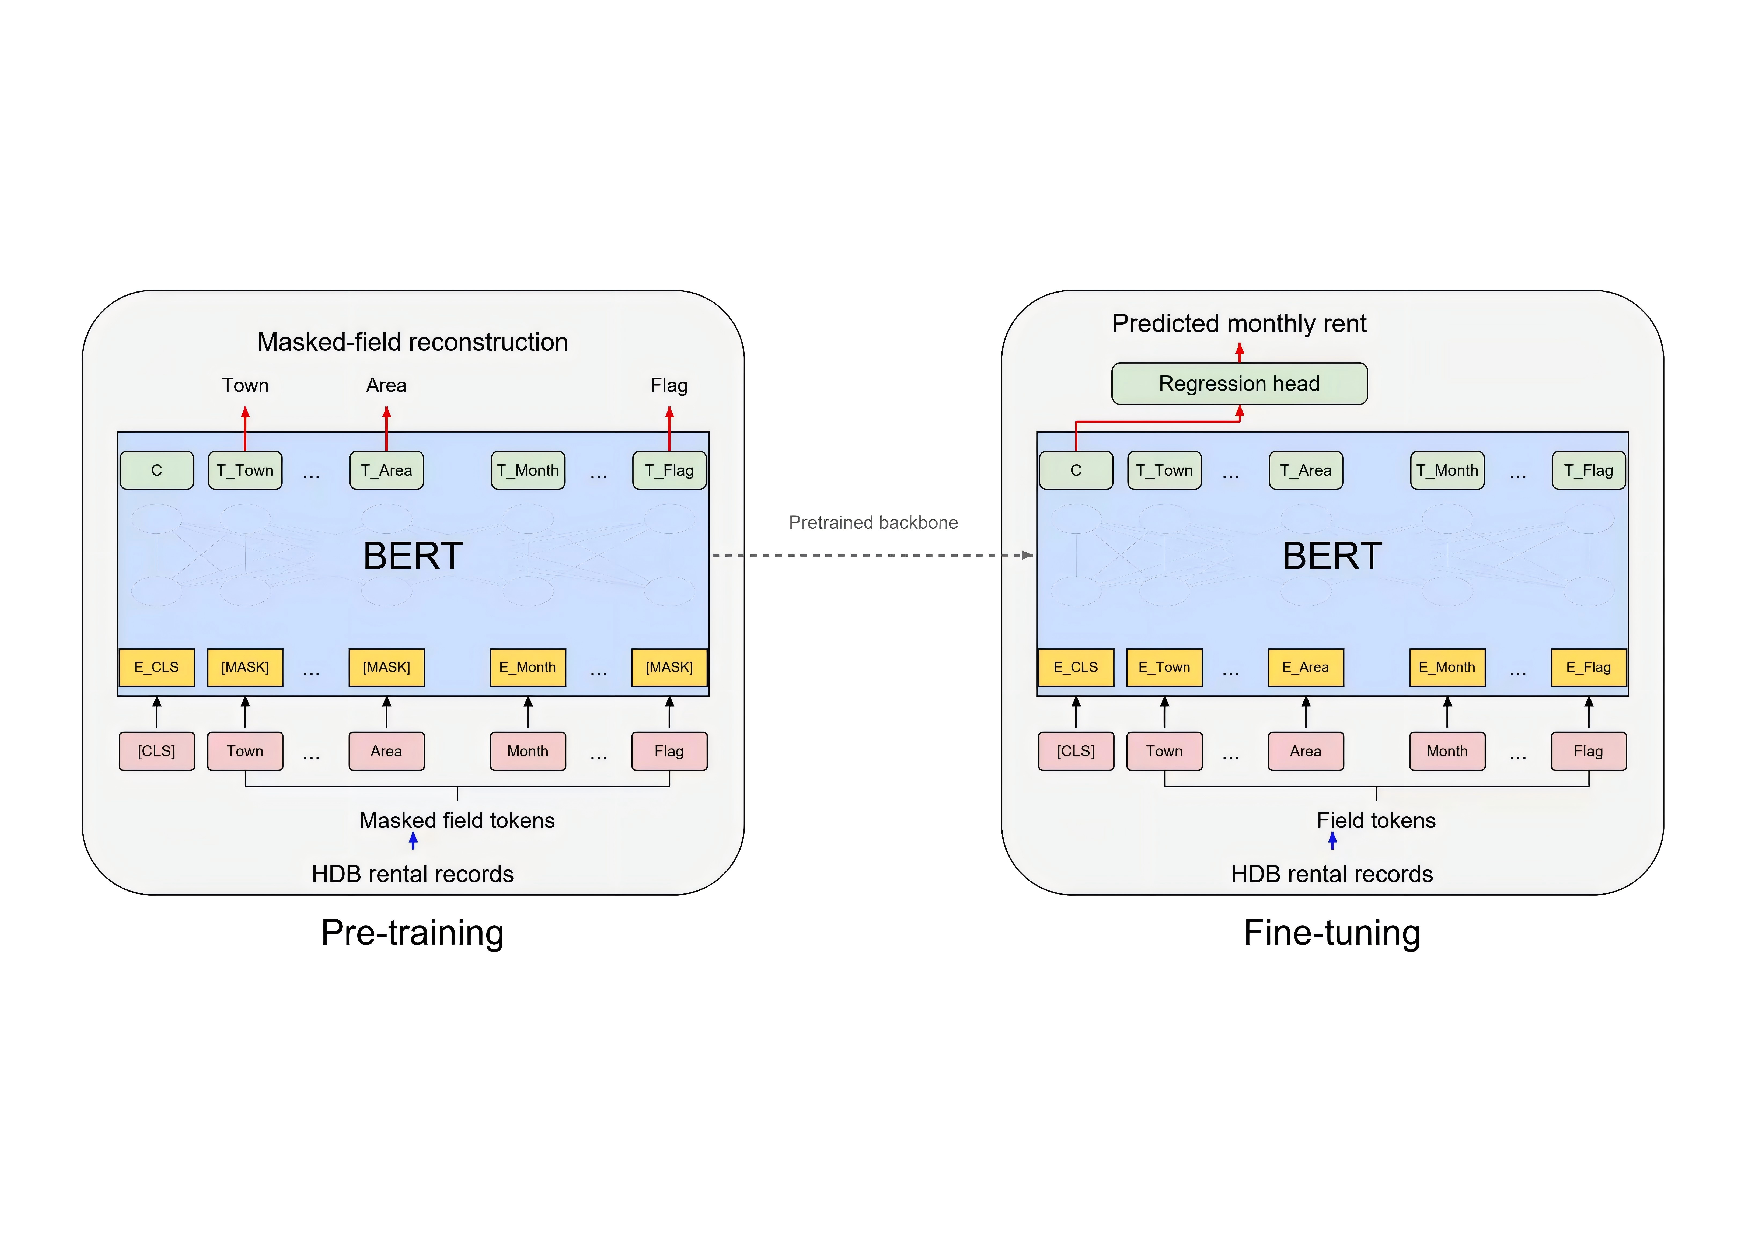
\includegraphics[width=0.9\textwidth]{fig_pretrain_finetune.pdf}
\caption{Overview of the two-stage procedure.  Left: during pretraining, randomly selected field tokens of an HDB rental record are replaced by \texttt{[MASK]} and the encoder reconstructs them (e.g., town, area, flag); rent is not used.  Right: the pretrained backbone is reused, and a regression head on the \texttt{[CLS]} output predicts the monthly rent.  Figure~\ref{fig:architecture} gives the layer-level details.}
\label{fig:pretrain_finetune}
\end{figure*}

\subsection{Related Work}
Dynamic hedonic models relate housing prices to property attributes while allowing these relationships to vary across time and municipalities~\cite{meese1991hedonic}.  Tabular-learning benchmarks find that tree methods remain competitive on medium-sized datasets, motivating a categorical-feature baseline such as CatBoost~\cite{grinsztajn2022trees,prokhorenkova2018catboost}.  Neural alternatives use different mechanisms: TabM builds parameter-efficient MLP ensembles~\cite{gorishniy2025tabm}, while TabPFN learns from synthetic tasks and predicts using labeled examples as context~\cite{hollmann2025tabpfn}.  ModernNCA learns representations for neighborhood-based prediction~\cite{ye2025modernnca}.  These three neural alternatives were considered but not run in this study.  Our experiments compare the recorded baselines and field-token BERT under future-month protocols, whose rankings must be checked on the rental data itself.
% Source: primary papers verified in reference_verification.md; ../../docs/research/PRIORITY_PLAN.md (unimplemented alternatives).

\subsection{Baselines and Design Rationale}
The comparison includes four baselines with increasing complexity.  The global mean uses the training-period rent average.  The recent grouped mean uses the latest six training months and averages by town and flat type, falling back to a flat-type mean and then a global mean when a group has fewer than ten observations.  Ridge~\cite{hoerl1970ridge} uses one-hot encodings for the eight categorical IDs with regularization strength 10, while shallow CatBoost~\cite{prokhorenkova2018catboost} uses the same 30 inputs, depth 4, 500 rounds, learning rate 0.1 and seed 42.  Its number of rounds is fixed without using validation labels.  Section~\ref{sec:evaluation} evaluates all four baselines under both protocols.

We selected a field-token encoder because self-attention can represent pairwise and higher-order interactions without imposing a linear effect for month, area or distance.  Masked-field reconstruction is intended to learn structure from labeled-period features without using rent labels.  Its incremental benefit remains untested because BERT was not evaluated without pretraining.
% Source: ../../results/baselines/round_a/README.md; ../../results/baselines/round_a/scores.csv; ../../docs/research/README.md; ../../docs/research/PRIORITY_PLAN.md; ../../report/PREPARATION.md.

\subsection{Field Tokenization and Encoder}
Each row contains 30 scalar inputs: eight categorical IDs, 19 standardized numeric fields, two calendar scalars and one imputation flag.  The two calendar values share one token, giving 29 field tokens.  Category IDs use learned embeddings (dimensions 16, 16, 32, 8, 8, 8, 8 and 8 in the configured field order) followed by a projection to width 768.  Each numeric field uses a separate $1\!\to\!32\!\to\!768$ network with GELU; the calendar pair uses a $2\!\to\!768$ projection and the flag a $1\!\to\!768$ projection.  A learned \texttt{[CLS]} vector is prepended, so the encoder sequence has length 30.

The backbone is a BERT encoder with 12 layers, hidden width 768, 12 attention heads, intermediate width 3072 and dropout 0.1.  The Hugging Face \texttt{BertModel} is instantiated from a configuration, with all encoder weights randomly initialized for this tabular task.  Fixed field order and positional embeddings identify which field each token represents.  Figure~\ref{fig:architecture} summarizes the token construction, encoder and the two training heads.
% Source: ../../src/bert_rent/model.py; ../../src/bert_rent/data.py; ../../configs/bert.json.

\begin{figure*}[t]
\centering
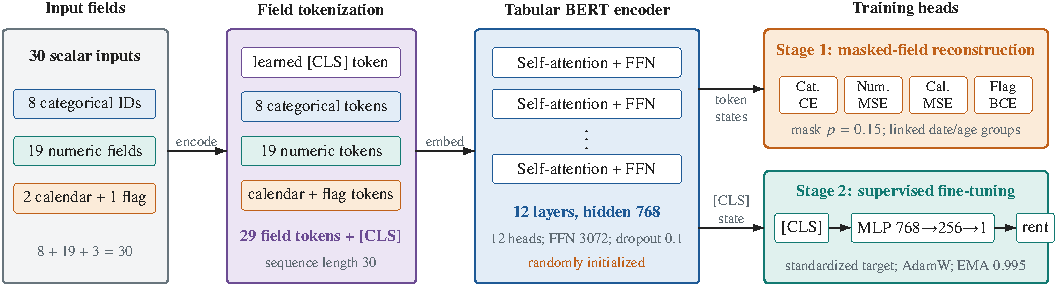
\includegraphics{model_architecture.pdf}
\caption{Two-stage field-token model.  Thirty scalar inputs form 29 field tokens and a learned \texttt{[CLS]} token.  Stage 1 reconstructs masked fields with type-specific heads; Stage 2 reads \texttt{[CLS]} with a rent regression head.  The encoder is randomly initialized BERT (12 layers, width 768, 12 heads).}
\label{fig:architecture}
\end{figure*}

\subsection{Masked-Field Pretraining}
For every training row, each field group is selected with probability 0.15 and at least one group is forced to be selected.  The selected token is replaced by a learned mask vector.  Two sets of mutually determined fields are masked jointly: \texttt{MONTH\_INDEX} with the calendar pair, and \texttt{LEASE\_COMMENCE\_DATE}, \texttt{AGE\_YEARS}, \texttt{YEAR\_COMPLETED} and \texttt{COMPLETION\_AGE}.  Joint masking prevents the reconstruction task from becoming a direct copy from a visible duplicate field.  The category heads use cross-entropy, numeric and calendar heads use mean squared error, and the flag head uses binary cross-entropy; the available type losses are averaged within type and summed.  Rent is not passed to this stage.
% Source: ../../src/bert_rent/model.py; ../../src/scripts/train_stage1_pretrain.py; ../../configs/bert.json.

\subsection{Rent Regression and Training Procedure}
For fine-tuning, the \texttt{[CLS]} representation is passed through LayerNorm, a 768-to-256 linear layer, GELU, dropout and a final scalar layer.  The target is standardized using the current training rows, mean squared error is optimized, and predictions are transformed back to SGD/month before scoring.  AdamW uses weight decay 0.01; the pretraining learning rate is $10^{-4}$, while fine-tuning uses $2\times10^{-5}$ for the encoder and $10^{-4}$ for the head.  The configured effective batch size is 1,024, gradient norm is clipped at 1.0, and the schedules use two or three warm-up epochs followed by cosine decay.  Fine-tuning maintains an exponential moving average with decay 0.995.  The recorded BERT runs use seed 42 and float32 arithmetic.

Training is separated into selection and refitting.  In the selection round, the first 39 labeled months (2021-01--2024-03) train the model and the last 12 labeled months select the epoch, with a patience of five epochs.  The recorded best epochs are 40 for masked-field pretraining and 7 for fine-tuning.  The refit round then trains on all 149,685 retained rows for exactly those epoch counts and does not use validation labels.  These values describe one frozen configuration with early stopping; they do not constitute a systematic hyperparameter search.
% Source: ../../src/bert_rent/engine.py; ../../src/scripts/train_stage1_pretrain.py; ../../src/scripts/train_stage2_finetune.py; ../../configs/bert.json; ../../results/split.json; ../../results/refit.json; ../../results/validation_summary.json.
